% !TeX program = xelatex
\documentclass[10pt,letterpaper]{article}
\usepackage[margin=.7in]{geometry}
\usepackage{graphicx,amsmath,fontspec,unicode-math}
\setmainfont{NimbusRoman-Regular.otf}[Path=../fonts/urw/,BoldFont=NimbusRoman-Bold.otf,ItalicFont=NimbusRoman-Italic.otf,BoldItalicFont=NimbusRoman-BoldItalic.otf]
\setsansfont{NimbusSans-Regular.otf}[Path=../fonts/urw/,BoldFont=NimbusSans-Bold.otf,ItalicFont=NimbusSans-Italic.otf,BoldItalicFont=NimbusSans-BoldItalic.otf]
\setmathfont{Latin Modern Math}
\usepackage[hidelinks]{hyperref}
\hypersetup{pdfauthor={},pdftitle={LoDA-SA: Current configuration and evidence}}
\graphicspath{{../figures/}}
\pagestyle{plain}
\setlength{\emergencystretch}{1em}
\begin{document}
\section*{LoDA-SA: Current configuration and evidence}
\section*{Supplementary Note S1: Current shared-coordinate configuration}
The selected operating point uses $(n_b,n_l)=(32,4096)$ with token quotas off, not a maximum selected independently from each benchmark. For Qwen3-8B split-half RoPE, $J=\{48,\ldots,63,112,\ldots,127\}$ contains 16 complete low-frequency pairs. One width-32 view serves both selection stages; original Q/K/V remain full-dimensional for final attention. Near and far scoring share the map. The extrema upper bound applies only in this view, not to original-dimensional logits or page attention mass. Pairing semantics do not automatically extend to learned projections, static-pair modes or MLA.

The reference path disables dynamic far gating, static layer skipping and L2 candidate gathering. L2 computes full-history logits before page masking, per-query-head softmax and KV-group probability averaging, using scale $1/\sqrt{128}$. Final selected-KV access is backend-dependent. Configuration labels in quality snapshots do not certify all runtime flags or a clean producer tree.

\section*{Supplementary Figure S2: Regional page allocation and single token pool}
\noindent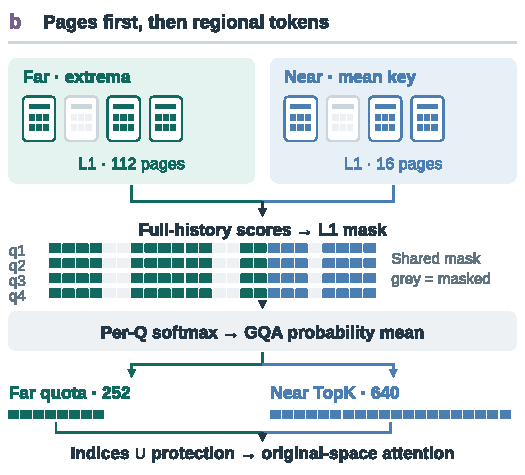
\includegraphics[width=.64\textwidth]{method_details/near_far_en.pdf}
\par\medskip\noindent Under sufficient eligible capacity, $K_1=128$ gives ranked-page quotas 32 near and 96 far. The 1024-token cap includes four sink and 128 recent tokens, leaving 892 nominal pooled slots when protection is disjoint. Boundary bypass pages enter outside ranked quotas; up to four protected prefix positions can be reselected, reducing distinct unprotected coverage. The blocks are schematic; per-query normalization precedes KV-group probability averaging.

\section*{Supplementary Note S3: Integer boundaries and support semantics}
\textbf{Integer boundaries and summary support.} In the current explicit-$n_l/n_b$ partitioned path, with $S=t+1$ valid cached positions including the current token and excluding padding, let $M=\max(0,S-s-w)$, $L=\max(B,n_l)$ and
\begin{align*}
b_n&=\max(\lfloor s/B\rfloor,\lfloor(S-w-L)/B\rfloor),\\
b_w&=\max(b_n,\lceil S/B\rceil-\max(1,\lfloor w/B\rfloor)).
\end{align*}
For sufficient history and disjoint protection, far and near L1 intervals before removing bypass pages are $[\lfloor s/B\rfloor,b_n)$ and $[b_n,b_w)$, respectively. The unified L2 interval is $[B\lfloor s/B\rfloor,S-w)$, with the combined page mask. Rounding and alignment can change near length from $n_l$. Summaries use full physical pages, not unprotected intersections: the partial prefix page includes protected keys, and the last near page can include recent-window keys at nonaligned $S$. Pooled L2 still stops at $S-w$. These rules exclude clustering, quota overrides and short-history branches.

\textbf{Scarce retained support.} In current unified selection, L1 page masking precedes L2 softmax. Pooled TopK clips counts to interval width, not positive support. If the clipped count exceeds that support, zero ties can select cached tokens from unselected pages; final selection does not reapply L1 eligibility. Figure~S2 assumes sufficient support and disjoint protection; partial-prefix reselection is separate. Occurrence and quality effects in the reported runs remain unverified.

\textbf{Fair comparison.} A matched comparison would require identical model, input IDs, generation limits and task scorer; equal-$K$ sparse comparisons count protection within the final unique cap. Retain and report each method's native phase, layer and protection policies; policy-matched adapters are separate controlled comparisons. Internal page caps may differ, but construction, scoring, ranking and traffic count toward complete-request cost. Report realized token counts and selection granularity, and match hardware and precision for timing.


\section*{Supplementary Note S4: Current-configuration evidence}
\textbf{Pooled-quality records (T6).} At revision \texttt{a7bcdddf}\allowbreak\texttt{727aa991}\allowbreak\texttt{96d925b9}\allowbreak\texttt{f106d785}\allowbreak\texttt{ce9273d4}, the manuscript input archive contains three T6 result JSONs, one for each length (32768, 65536 and 131072); their filenames use the prefix \texttt{t6\_ruler\_q8b\_L} and suffix \texttt{\_champ.json}. Their 11-task arithmetic means are 59.0209, 47.8000 and 46.8164; differences from the existing dense anchors are $-0.3609$, $-0.7364$ and $+0.3845$ points. Every task records $n=100$, with no incomplete cells. The source-defined labels bind $B=64$, $K_1=128$, $K=1024$, compression ratio 4, 4/128 protection and $(n_b,n_l)=(32,4096)$ with token quotas off. Provenance notes batch sizes 8/2/2 and YaRN off/2/4 across lengths. The snapshots store prediction-file hashes, not matching scorer, source-input or full effective-configuration manifests; those hashes cannot establish paired data or execution identity. The exact reported configuration string is \texttt{tli\_64\_128\_1024\_c4\_\allowbreak Aa0\_b0\_g1\_\allowbreak sk4\_sw128\_\allowbreak np32\_ntoff\_nl4096}. The three result JSONs are available in the versioned manuscript directory \texttt{figures/ruler32k\_comparison/inputs/}. Each result binds task scores, counts and prediction-file SHA-256 values. Separate receipts binding producer script, seed and generation identity have not been recovered in this inspected tree; those fields are not certified here. The following table retains all 11 task scores, with columns explicitly denoting lengths. No paired uncertainty or dense execution matching follows from these result records.
\begin{center}\small
\begin{tabular}{lrrr}\hline
Task & 32K & 64K & 128K \\ \hline
niah\_single\_1 & 100.00 & 94.00 & 97.00 \\
niah\_single\_2 & 100.00 & 100.00 & 100.00 \\
niah\_single\_3 & 100.00 & 100.00 & 99.00 \\
niah\_multikey\_1 & 98.00 & 99.00 & 99.00 \\
niah\_multikey\_2 & 71.00 & 39.00 & 39.00 \\
niah\_multikey\_3 & 7.00 & 0.00 & 0.00 \\
niah\_multiquery & 24.50 & 22.50 & 17.00 \\
niah\_multivalue & 28.50 & 36.00 & 3.75 \\
cwe & 74.10 & 0.30 & 0.70 \\
fwe & 15.33 & 5.00 & 37.33 \\
vt & 30.80 & 30.00 & 22.20 \\
\hline\end{tabular}
\end{center}


\textbf{Graph execution records (E152v4).} The same revision archives \texttt{exp/trace/results/}\allowbreak\texttt{e152v4\_formal\_pc40/} and its verdict. Recomputed dense/TLI Graph mean TPOTs are 26.282/24.702, 39.670/27.398 and 67.035/32.425 ms at nominal 32K/64K/128K. For example, the 128K timing record contains 134923 input tokens after prompt construction. The protocol reports Qwen3-8B BF16 on H20-3e, batch one, ABBA process ordering, two processes per arm and fixed 128-token output; dense has six measured repeats and Graph four per length. Per-step synchronization and argmax are included. Graph TPOT divides the post-cache-fill decode wall by 127, excluding static-cache filling and warmup capture. It does not report a preparation-inclusive request wall. The six dense files instead use the E152 v2 schema, DynamicCache and post-first-output timing; their records do not establish Graph execution. Although the later Graph script supports both arms, that capability cannot relabel these saved dense runs. Both arms mark backend verification false, and the declared runtime checkout does not supply the archived producer script, so exact runtime producer identity remains unresolved. The published v2 script calls model forward in a loop, not \texttt{generate}; this is inspected code, not complete runtime verification. Graph/eager token agreement is reported on the timing prompt, not benchmark-wide equivalence or equality to FullKV. The Graph treatment agrees with the T6 labels on the explicit budgets above, but T6 lacks a full frozen manifest and uses different batches. Neither the quality/timing records nor their speed ratios define a matched quality--cost frontier.

\textbf{Environment scope.} The verdict designates the primary H20-3e environment before its length-wise summary. All its measured runs are used. A separate local-GPU1 replica reports dense/sparse Graph TPOTs of 39.338/47.605, 59.250/51.572 and 77.831/66.513 ms at 32K/64K/128K (six/four measured runs per length). The 32K dense/sparse ratio is .826: the selected method is slower in that record. The source labels this replica co-tenant-polluted; independent interference logs have not been verified, so that attribution is reported rather than established. These results are not pooled across environments and do not support a hardware-independent acceleration claim.

\textbf{Cross-model execution diagnostics (E159/E160).} Table~II in the main text is recomputed from raw records at revision \texttt{906d8121}\allowbreak\texttt{9a2f55ec}\allowbreak\texttt{f7a73d18}\allowbreak\texttt{51ccb966}\allowbreak\texttt{55c0b585}. Under \texttt{exp/trace/results/}, E159 uses \texttt{e159\_\allowbreak llama/}\allowbreak\texttt{e159\_\allowbreak phase1\_\allowbreak v2\_\allowbreak pc40.json} for dense eager and \texttt{e159\_\allowbreak phase2\_\allowbreak graph\_\allowbreak pc40.json} for sparse Graph. E160 uses the \texttt{dense\_\allowbreak L\{32768,65536\}\_\allowbreak b\{1,2\}.json} and corresponding \texttt{tli\_\allowbreak graph\_\allowbreak L\{32768,65536\}\_\allowbreak a\{1,2\}.json} records in \texttt{e160\_\allowbreak 32b/}. Means exclude marked warmups and weight measured runs equally. Each row has matching recorded 16-hex-digit input-hash prefixes across arms; full hashes and a complete input/model/tokenizer manifest are not supplied. E159 draws its two arms from separate phase archives, not one verified cross-mode interleaving. Llama has six measured runs per arm/length; Qwen3-32B has six dense and four sparse runs. These repeats share a timing prompt, not independent task examples. A second-device Qwen3-32B record (\texttt{e160r\_\allowbreak 32b/}) gives dense/sparse means 55.582/54.685 and 80.414/59.969 ms at 32K/64K, respectively; it is a replication of timing, not quality.

The configured route is BF16 Hugging Face/PyTorch SDPA on H20-3e with Torch 2.8.0 and Transformers 4.56.2, not a verified production-serving backend. Sparse labels bind $K_1=128$, $K=1024$, compression ratio 4, 4/128 protection, near pages/extent $(32,4096)$ and token quotas off. Source provenance reports a shadow implementation, so a checkout identifier alone does not fix the executed code. Sparse TPOT measures the 127 post-fill decode intervals, including synchronization and argmax but excluding prefill, cache filling and Graph capture. Dense uses eager post-first-output timing. Thus the table compares execution regimes, not equally optimized Graph backends. The E159 dense-Graph path is markedly slower than dense eager; its 14.28 ratio at 128K is not used as evidence of the selector's advantage. Llama Graph/eager output agreement is checked only on a separate 16362-token smoke prompt. Qwen3-32B saved Graph/eager token arrays agree on the timing prompts; neither output-agreement check establishes task quality against FullKV.

\textbf{Qwen3-32B 128K protocol change (E160b).} The table's final row uses \texttt{e160b\_\allowbreak 128k/remote\_\allowbreak e160b/}: two \texttt{dense\_\allowbreak L131072\_\allowbreak b\{1,2\}.json} records and four \texttt{tli\_\allowbreak graph\_\allowbreak L131072\_\allowbreak a\{1,2,3,4\}.json} records. Both arms enable the expandable-segment allocator. Sparse runs use four separate processes, each with one measured run and no discarded warmup; capture occurs in that run but lies outside its reported TPOT. Dense retains one warmup and three measured runs per process. Recomputed means are 129.100739/70.109988 ms, with ratio 1.841403; statistical equivalence to the earlier repetition protocol is not established. All four sparse outputs match the single eager output-agreement run. Actual prompt length is 134923, exceeding the nominal 131072 label; the logs also warn about this length, and the result does not validate long-context quality. In the original E160 logs, warmup decoding succeeds before the next prefill fails with an out-of-memory error. The source report states that a repeated-run attempt with expandable segments also fails after successful warmup; the single-run-process records establish a narrower feasible execution, not a general memory-capacity guarantee. No preparation-inclusive request savings or matched quality--cost frontier follows from these timings.


\end{document}
